\chapter{Тестирование и аппробация плагина в Jenkins} \label{ch4}

% не рекомендуется использовать отдельную section <<введение>> после лета 2020 года
%\section{Введение. Сложносоставное название первого параграфа первой главы для~демонстрации переноса слов в содержании} \label{ch1:intro}

При разработке плагина надо было учитывать, что требуется отображать все графики на одной странице задания друг под другом, поскольку при выборе одно периода, например, месяца, будет получена сводная информация по каждой сборке или нескольких сборок запущенных в один день. Графики отображаются посредством переходна на соотвествующую ссылку, оставляя при этом пользователя в том же задании (странице с результатами последних сборок).

В интерфейсе у каждого графика были реализованы те дополнительные функции отображения, которые могут быть применины к визуализируемой метрике: отобразить статистику по упавшим сборкам/тестам, усреднить метрику.

Интерфейс страницы плагина с графиками в системе Jenkins на странице задания показан на рисунке 3.1.


\begin{figure}[ht!] 
	\center
	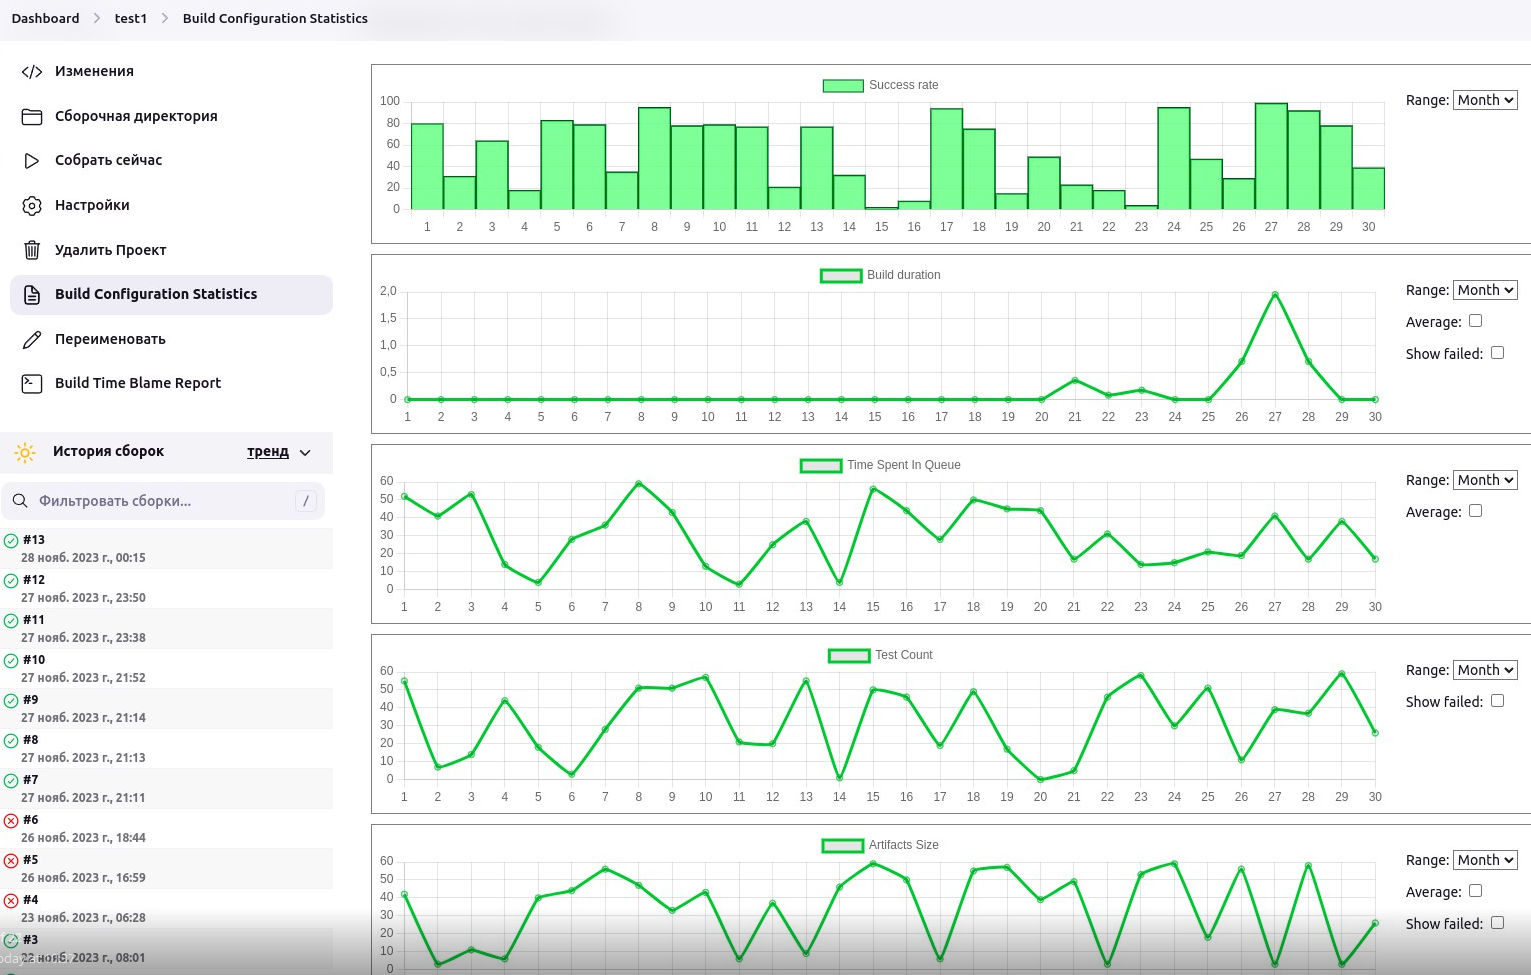
\includegraphics [scale=0.47] {my_folder/images//ui}
	\caption{Интерфейс плагина Jenkins} 
	\label{fig:ArchitectureJenkins}  
\end{figure}

Основное взаимодействие с графиками будет производить через меню, которое есть напротив каждого графика со своими параметрами, отображенном на рисунке 3.2:

\begin{figure}[ht!] 
	\center
	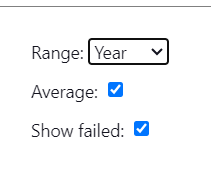
\includegraphics [scale=0.47] {my_folder/images//ui2}
	\caption{Интерфейс элементов управления} 
	\label{fig:ArchitectureJenkins}  
\end{figure}

При взаимодействии с раскрывающимся списком должен вызываться Java метод, который пересчитает и отфильтрует необходимые сборки Jenkins и динамически отобразит результаты по выбранными периоду, также динамически должна производить обработка метрик сборок, при выборе основной метрики ни как суммы всех значений, а как среднего, а также включение в графики данных об упавших сборках, при выборе соотвествующих чекбоксов.

Интерфейс изменения навигационной панели отображен на рисунке 3.3. В данном случае видно что изменения видны при открытии конфигурации конкретной сборки, т.е. не надо будет переключаться между окном плагина и сборкой для визуализации метрик, при открытии данного пункта меню, также происходит изменения URL, с которым в дальнейшем и происходит взаимодействие.

\begin{figure}[ht!] 
	\center
	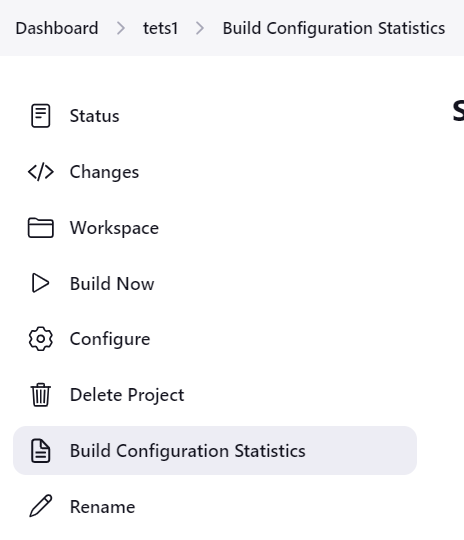
\includegraphics [scale=0.47] {my_folder/images//ui3}
	\caption{Интерфейс элементов управления} 
	\label{fig:ArchitectureJenkins}  
\end{figure}



Код плагина представлен в приложении 4.
 






%
%

%
%
%\begin{table} [htbp]% Пример оформления таблицы
%	\centering\small
%	\caption{Представление данных для сквозного примера по ВКР \cite{Peskov2004}}%
%	\label{tab:ToyCompare}		
%		\begin{tabular}{|l|l|l|l|l|l|}
%			\hline
%			$G$&$m_1$&$m_2$&$m_3$&$m_4$&$K$\\
%			\hline
%			$g_1$&0&1&1&0&1\\ \hline
%			$g_2$&1&2&0&1&1\\ \hline
%			$g_3$&0&1&0&1&1\\ \hline
%			$g_4$&1&2&1&0&2\\ \hline
%			$g_5$&1&1&0&1&2\\ \hline
%			$g_6$&1&1&1&2&2\\ \hline		
%		\end{tabular}	
%	\normalsize% возвращаем шрифт к нормальному
%\end{table}


% \firef{} от figure reference
% \taref{} от table reference
% \eqref{} от equation reference




